\documentclass[12pt,a4paper]{article}

\usepackage[utf8]{inputenc}
\usepackage{graphicx}
\usepackage{float}

\begin{document}

\title{MI-PAA 2015 1.ukol}
\author{Tomas Nesrovnal\\nesrotom@fit.cvut.cz}
\date{\today}
\maketitle

\section{Specifikace ulohy}
Problem batohu.

\section{Rozbor moznych variant reseni}
Ulohu muzu resit hrubou silou. Ziskam tam presny vysledek, ale vypocet bude
pomaly. Dalsim resenim je pouzit heuristiku, jejiz vyledek nebude nejlepsi mozny
ale vypocet probehne rychle.

\section{Ramcovy popis postupu reseni}
\subsection{Hruba sila}
Zkusim vsechny moznosti a vyberu tu nejlepsi.
\subsection{Heuristika}
Vkladam do bahothu nejlepsi predmety s pomerem cena/vaha, dokud
mi jeste staci kapacita.

\section{Popis kostry algoritmu}
\subsection{Hruba sila}
Vytvorim pole, ktere udava ktery predmet je v batohu. Rekurzivne zkousim
vsechny moznosti (zavolam rekurzi bez prvku, pak prvek pridam a zavolam rekurzi znovu).
Ulozim si nejlepsi reseni.

Pokud ve stromu reseni narazim na to, ze se do batohu uz vic nevejde, vetev zariznu.
\subsection{Heuristika}
Seradim si pole s predmety podle pomeru cena/vaha (nebo jine varianty, viz grafy). Cele pole sestupne prochazim a pokud se tam predmet vejde, tak ho tam vlozim.

\section{Namerene vysledky}

\subsection{Spravnost vysledku}
Pomoci skriptu byla overena spravnost vysledku (porovnanim s referencnim resenim).

\subsection{Na cem bylo mereno}
Intel(R) Core(TM) i3-2328M Processor (3M Cache, 2.20 GHz), gcc 4.9.2 (-Ofast), OS GNU/Linux Lubuntu 14.04 64bit

\subsection{Grafy}
Grafy byly vygenerovany skripty (tests/run.sh a time.sh). Cas byl meren pomoci knihovny OpenMPI.

Presna cisla lze nalezt v .plot souborech.

Chyba heuristiky: Z kazdeho batohu spocitana relativni chyba. V grafu jsou pak secteny relativni chyby pro celou sadu. Celkem 4 heuristiky.

\begin{figure}[H]
	\caption{Doba behu reseni heuristikou (cena/vaha). 50k opakovani. (cas je v sekundach)}
	\includegraphics{./time_h.png}
\end{figure}

\begin{figure}[H]
	\caption{Doba behu reseni hrubou silou. Pouze jedno opakovani, presto instance o 32 dvou prvcich trvala 22 minut. (cas je v sekundach) }
	\includegraphics{./time_b.png}
\end{figure}

\begin{figure}[H]
	\caption{heuristika (podle ceho se radilo): pomer cena/vaha}
	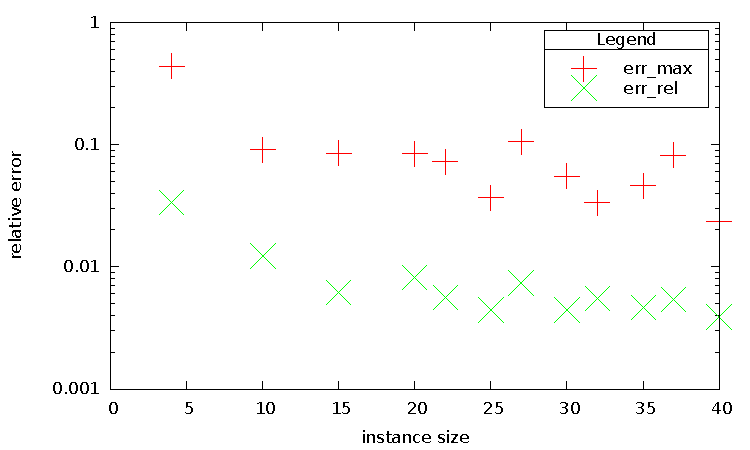
\includegraphics{./err_h1.pdf}
\end{figure}

\begin{figure}[H]
	\caption{heuristika (podle ceho se radilo): pomer vaha/cena}
	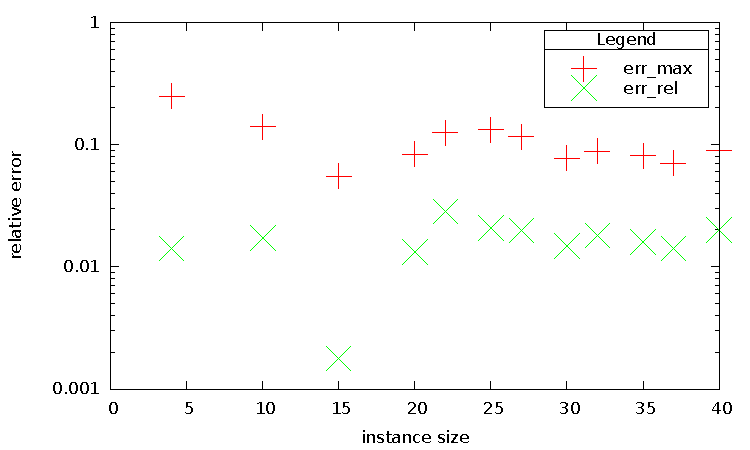
\includegraphics{./err_h2.pdf}
\end{figure}

\begin{figure}[H]
	\caption{heuristika (podle ceho se radilo): cena}
	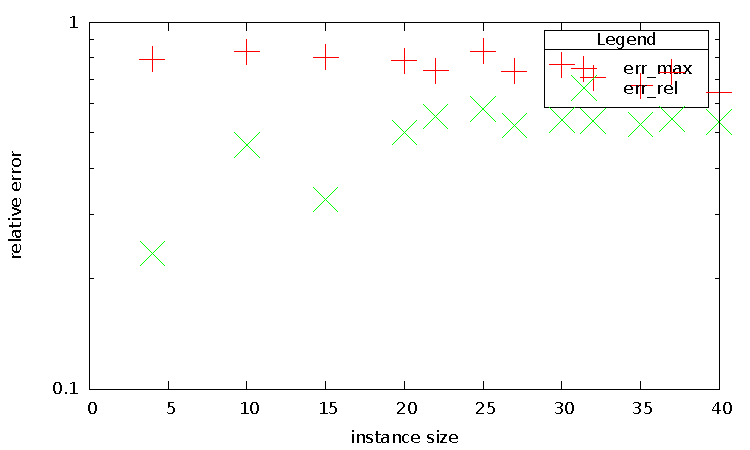
\includegraphics{./err_h3.pdf}
\end{figure}

\begin{figure}[H]
	\caption{heuristika (podle ceho se radilo): vaha}
	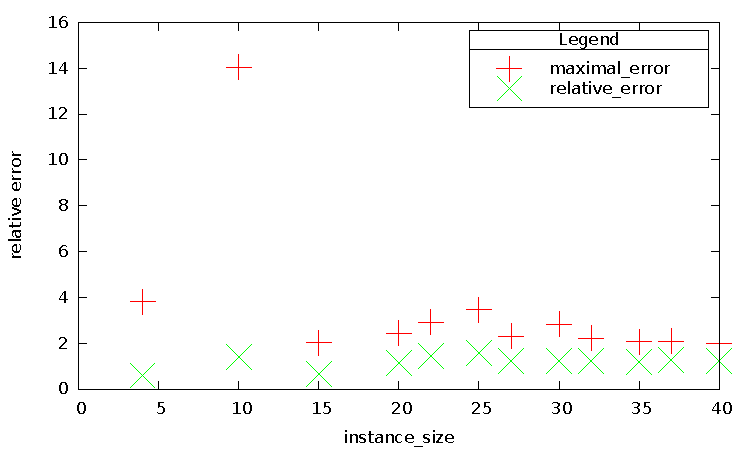
\includegraphics{./err_h4.pdf}
\end{figure}

\section{Zaver}
Vysledky se shoduji s rozborem reseni. Hruba sila je opravdu pomala a byt jednoducha heuristika nevraci zas tak spatne reseni.

Heuristika cena/vaha byla nejlepsi z heuristik.
\end{document}
